\chapter{Cálculo de la aniquilación $SS\rightarrow Z^0Z^0$}
Author: Sebastian Bustamante

Descripcion del proceso: 

\section{Descripción del proceso.}

La aproximación usada en \cite{Goud} para la materia oscura corresponde a un singlete escalar que solo está acoplado con el Higgs del modelo estándar, el lagrangiano más general que describe esta partícula es por tanto
\eq{1}
{ \mathcal{L} = \mathcal{L}_{SM} + \frac{1}{2}\partial_\mu S\partial^\mu S - \frac{m_0^2}{2}S^2 - \frac{\lambda_S}{4}S^4 - \lambda S^2 H^\dag H }
donde $S$ es el campo escalar propuesto, $m_0$ la masa del campo y $\lambda$ es un parámetro que caracteriza el acople con el Higgs.

Del lagrangiano del modelo estándar \cite{profe}, los únicos estados finales por decaimiento de este campo $S$ a través del canal s son $f\bar f$, $W^+W^-$, $Z^0Z^0$ y $hh$. En especial en este documento se calculará todo lo referente al proceso $SS\rightarrow Z^0Z^0$, para el cual el diagrama de Feynmann asociado es

\begin{figure}[htbp]
	\centering
	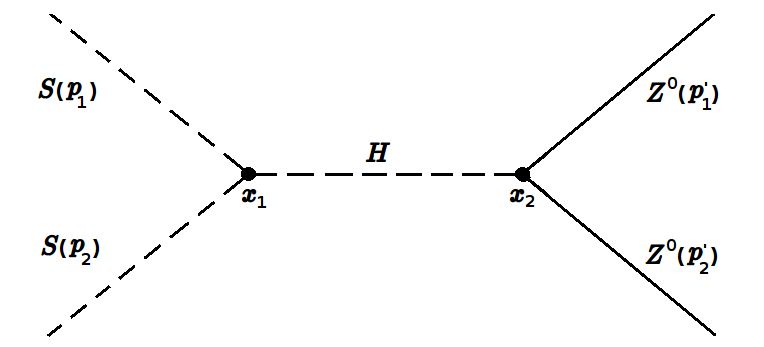
\includegraphics[width=0.5\textwidth]{Sebastian_fig01.png}
	\caption{Diagrama de Feynmann para el proceso $SS\rightarrow Z^0Z^0$.}
	\label{fig:fig01}
\end{figure}

Puesto que el proceso es a través del canal s este debe tener dos vértices, tal como se ve en el diagrama anterior.

\section{Lagrangiano del proceso}

El único término de interés del lagrangiano de interacción del modelo estándar es aquel que acopla dos bosones $Z^0$ con un higgs, este está dado por \cite{profe}
\eq{2}
{ \mathcal{L}_{SM,I} = \frac{m_Z^2}{v} Z^2 h }
y por tanto el lagrangiano de interacción total es
\eq{3}
{ \mathcal{L}_{T} = \frac{m_Z^2}{v} Z^2 h - \lambda S^2 H^\dag H   }
donde por simplicidad en notación se ha hecho $Z\equiv Z^0$.

Se hace conviente introducir el doblete de higgs del modelo estándar de la forma
\[ H = \frac{1}{\sqrt 2}
\begin{pmatrix}
  0 \\\ h(x) + v
\end{pmatrix} \]
de esto
\[ H^\dag H = \frac{1}{2}\pr{ v^2 + hh + 2vh } \]
y luego
\[ \mathcal{L}_{T} = \frac{m_Z^2}{v} Z^2 h - \frac{\lambda }{2}S^2\pr{ v^2 + hh + 2vh }  \]
Teniendo en cuenta el estado inicial del proceso en estudio, se tiene que solo es interesante el término de acople de $S^2$ con un higgs $h$, por tanto el lagrangiano de interacción relevante para los cálculos que serán realizados es finalmente
\eq{4}
{ \mathcal{L}_{I} = \frac{m_Z^2}{v} Z^2 h - \lambda vS^2 h  }
como no hay dependencia en las derivadas de los campos, el hamiltoniano de interacción es
\eq{5}
{ \mathcal{H}_{I}(x) = \mathcal H_1(x) + \mathcal H_2(x) }
donde se han definido los hamiltonianos
\[ \mathcal H_1(x) \equiv \lambda vS(x)S(x) h(x) \ \ \ \ \ \ \ \ \ \ \mathcal H_2(x) \equiv -\frac{m_Z^2}{v} Z(x)Z(x) h(x)   \]
Puesto que ninguno de los tres hamiltonianos exhibe acople entre las tres partículas simultáneamente, se concluye que el primer orden de la matriz $S$ no contribuye al proceso, tan solo lo hace el segundo orden. Esto es equivalente a decir que el proceso es de dos vértices, tal como se ha mostrado en la sección anterior.

\section{Matriz S}
De la discusión anterior, se procede entonces a calcular el segundo orden de la matriz $S$
\[ S^{(2)} = \frac{(-i)^2}{2!}\int dx_1^4 \int dx_2^4 \mathcal{T}\cor{ :\mathcal H_I(x_1):\ :\mathcal H_I(x_2): } \]
expandiendo el argumento del operador de ordenamiento espacio-temporal se obtiene
\[ :\mathcal H_I(x_1):\ :\mathcal H_I (x_2): \ = \]
\[:\mathcal H_1 (x_1):\ :\mathcal H_1 (x_2): + :\mathcal H_1 (x_1):\ :\mathcal H_2 (x_2): + :\mathcal H_2 (x_1):\ :\mathcal H_1(x_2): + :\mathcal H_2 (x_1):\ :\mathcal H_2 (x_2): \]
de la figura (\ref{fig:fig01}) y de la definición de cada hamiltoniano es claro que solo el segundo término contribuye al proceso deseado, por tanto
\[S^{(2)} = \frac{(-i)^2}{2!}\int dx_1^4 \int dx_2^4 \mathcal{T}\cor{ :\mathcal H_1(x_1):\ :\mathcal H_2(x_2): } \]
introduciendo la forma explícita de $\mathcal H_1 y \mathcal H_2$
\eq{6}
{ \bcontraction{S^{(2)} = -\frac{(-i)^2}{2!}\lambda m_Z^2\int dx_1^4 \int dx_2^4 \mathcal{T}[:[S^2\ }{h}{](x_1):\ :[Z^2}{h}
S^{(2)} = -\frac{(-i)^2}{2!}\lambda m_Z^2\int dx_1^4 \int dx_2^4 \mathcal{T}\cor{ :[S^2h](x_1):\ :[Z^2h](x_2): } }
Donde la contracción de Wick se hace sobre el higgs puesto que es la partícula mediadora del proceso.

Introduciendo los operadores de creación y aniquilación, 
\[ Z = Z^+ + Z^- \ \ \ \ \ \ \ \ \ \ \ \ \ \ \ \ S = S^+ + S^-\]
y el producto ordenado del integrando de la matriz $S^{(2)}$ queda
\[ \bcontraction{ \mathcal{T}[:[S^2\ }{h}{](x_1):\ :[Z^2}{h}  \bcontraction{\mathcal{T}\cor{ :[S^2h](x_1):\ :[Z^2h](x_2): } = }{h}{(x_1)}{h}    \mathcal{T}\cor{ :[S^2h](x_1):\ :[Z^2h](x_2): } = h(x_1)h(x_2)Z_1^-(x_2)Z_2^-(x_2)S_1^+(x_1)S_2^+(x_1) \]
donde los subíndices en los operadores de aniquilación y creación indican la partícula $1$ o $2$.

\newpage

Teniendo en cuenta que la contracción de Wick del anterior campo escalar es proporcional al propagador
\[ \bcontraction{}{h}{(x_1)}{h}  h(x_1)h(x_2) = i\Delta_F(x_1-x_2)  \]
La matriz $S^{(2)}$ queda finalmente
\eq{7}
{S^{(2)} = -\frac{(-i)^2}{2!}\lambda m_Z^2\int dx_1^4 \int dx_2^4 i\Delta_F(x_1-x_2)Z_1^-(x_2)Z_2^-(x_2)S_1^+(x_1)S_2^+(x_1) }
Calculando el elemento de matriz asociado al proceso
\[ S^{(2)}_{fi} = \bra f|S^{(2)}|i\ket = \bra Z^0(p_1') Z^0(p_2') | S^{(2)} | S(p_1) S(p_2) \ket \]
con las siguiente relaciones
\[ | S(p_1) \ket = \sqrt{\frac{2\pi^3}{V}}\hat a^\dag _{p_1}|0\ket \ \ \ \ \ \ \ \ | S(p_2) \ket  = \sqrt{\frac{2\pi^3}{V}}\hat a^\dag _{p_2}|0\ket \]
\[ | Z^0(p_1') \ket = \sqrt{\frac{2\pi^3}{V}}\hat b^\dag _{p_1'}|0\ket \ \ \ \ \ \ \ \ | Z^0(p_2') \ket = \sqrt{\frac{2\pi^3}{V}}\hat b^\dag _{p_2'}|0\ket \]
donde $\hat a_{p}$ es un operador que crea una partícula $S$ con momentum $p$, y $\hat b_{p'}$ crea un bosón $Z^0$ con momentum $p'$.

El elemento de matriz queda entonces
\[ S^{(2)}_{fi} =-\frac{(-i)^2}{2!}\lambda m_Z^2\int dx_1^4 \int dx_2^4 i\Delta_F(x_1-x_2)\times\]
\[\bra Z^0(p_1') Z^0(p_2') |Z_1^-(x_2)Z_2^-(x_2)S_1^+(x_1)S_2^+(x_1)| S(p_1) S(p_2) \ket \]
y teniendo en cuenta que 
\[ S^+(x) = \sqrt{\frac{V}{2\pi^3}}\int \frac{d^4k}{\sqrt{2E_k V}}e^{-ik\cdot x} \hat a_{k} \]
se obtiene
\eq{10}
{ S_1^+(x_1)S_2^+(x_1)| S(p_1) S(p_2) \ket = \int \frac{d^4k'}{\sqrt{2E_{k'} V}} \int \frac{d^4k}{\sqrt{2E_k V}}e^{-ik'\cdot x_1}e^{-ik\cdot x_1} \hat a_{k} \hat a_{k'}\hat a^\dag _{p_1}\hat a^\dag _{p_2}|0\ket }
Para simplificar esto se calcula el siguiente conmutador
\[ [ \hat a_{k}\hat a_{k'},\hat a^\dag _{p_1}\hat a^\dag _{p_2} ] \]
expandiendo según la identidad
\[ [AB,CD] = AC[B,D] + A[B,C]D + C[A,D]B + [A,C]DB \]
y la relación de conumtación bosónica
\[ [\hat a_{p}, \hat a^\dag _{p'}] = \delta(p-p') \]
se llega a 
\eq{8}
{ [ \hat a_{k}\hat a_{k'},\hat a^\dag _{p_1}\hat a^\dag _{p_2} ] = \hat a_{k}\hat a^\dag _{p_1}\delta( k' - p_2 ) + \hat a_{k} \hat a^\dag _{p_2} \delta( k' - p_1 ) + \hat a^\dag _{p_1}\hat a_{k'}\delta( k-p_2 ) + \hat a^\dag _{p_2}\hat a_{k'}\delta(k - p_1) }
Recordando que un operador de aniquilación actuando sobre el estado de vacío da un efecto nulo, se concluye que
\[ [ \hat a_{k}\hat a_{k'},\hat a^\dag _{p_1}\hat a^\dag _{p_2} ]|0\ket = \hat a_{k}\hat a_{k'}\hat a^\dag _{p_1}\hat a^\dag _{p_2} |0\ket \]
usando (\ref{eq8})
\[ \hat a_{k}\hat a_{k'}\hat a^\dag _{p_1}\hat a^\dag _{p_2} |0\ket = \delta( k' - p_2 )\hat a_{k}\hat a^\dag _{p_1}|0\ket + \delta( k' - p_1 )\hat a_{k} \hat a^\dag _{p_2} |0\ket \]
y aplicando los operadores sobre el estado del vacío, se llega a
\eq{9}
{ \hat a_{k}\hat a_{k'}\hat a^\dag _{p_1}\hat a^\dag _{p_2} |0\ket = \delta( k' - p_2 )\delta(k-p_1)|0\ket + \delta( k' - p_1 )\delta(k-p_2) |0\ket }

\newpage

Con (\ref{eq9}) es fácil evaluar (\ref{eq10}), quedando
\eq{11}
{ S_1^+(x_1)S_2^+(x_1)| S(p_1) S(p_2) \ket =  \frac{1}{\sqrt{2E_{p_2} V}} \frac{1}{\sqrt{2E_{p_1} V}}2e^{-ip_2\cdot x_1}e^{-ip_1\cdot x_1} |0\ket }
Asumiendo que el bosón $Z^0$ está polarizado puede tomarse como un escalar, por tanto el resultado anterior es igualmente valido para este
\eq{11}
{ \bra Z^0(p'_1) Z^0(p'_2) |Z_1^-(x_2)Z_2^-(x_2) = \bra 0 | \frac{1}{\sqrt{2E_{p'_2} V}} \frac{1}{\sqrt{2E_{p'_1} V}}2e^{ip'_2\cdot x_2}e^{ip'_1\cdot x_2} }

\

El elemento de matriz de $S^{(2)}$ queda
\[ S^{(2)}_{fi} =-4\frac{(-i)^2}{2!}\lambda m_Z^2\cor{\frac{1}{\sqrt{2E_{p'_2} V}} \frac{1}{\sqrt{2E_{p'_1} V}}\frac{1}{\sqrt{2E_{p_2} V}} \frac{1}{\sqrt{2E_{p_1} V}}}\times \] \[
\int dx_1^4 \int dx_2^4 i\Delta_F(x_1-x_2) e^{-ip_2\cdot x_1}e^{-ip_1\cdot x_1}e^{ip'_2\cdot x_2}e^{ip'_1\cdot x_2} \]
Introduciendo la transformada de Fourier inversa del propagador
\[ \Delta_F(x)  = \int\frac{d^4q}{(2\pi)^4}\Delta_F(q)e^{iq \cdot x}  \]
\[ S^{(2)}_{fi} =-4\frac{(-i)^2}{2!}\lambda m_Z^2\cor{\frac{1}{\sqrt{2E_{p'_2} V}} \frac{1}{\sqrt{2E_{p'_1} V}}\frac{1}{\sqrt{2E_{p_2} V}} \frac{1}{\sqrt{2E_{p_1} V}}}\times \] \[
\int dx_1^4 \int dx_2^4 \int\frac{d^4q}{(2\pi)^4}i\Delta_F(q)e^{iq \cdot (x_1-x_2)} e^{-ip_2\cdot x_1}e^{-ip_1\cdot x_1}e^{ip'_2\cdot x_2}e^{ip'_1\cdot x_2} \]
Recordando la transformada de la delta de dirac
\[ \delta^4( p-p' ) = \frac{1}{(2\pi)^4}\int d^4 x e^{-i(p-p')\cdot x} \]
y usando 
\[ \delta(q-x)\delta(q-y) = \delta( q-x )\delta(x-y) \]
se obtiene finalmente
\[ S^{(2)}_{fi} =-4\frac{(-i)^2}{2!}\lambda m_Z^2\cor{\frac{1}{\sqrt{2E_{p'_2} V}} \frac{1}{\sqrt{2E_{p'_1} V}}\frac{1}{\sqrt{2E_{p_2} V}} \frac{1}{\sqrt{2E_{p_1} V}}}\times \] 
\eq{13}
{ (2\pi)^4\delta^4(p_1+p_2-p'_1-p'_2)i\Delta_F( p_1 + p_2 ) }
De la relación definitoria de la matriz $\mathcal{M}_{fi}$ \cite{lah}
\eq{14}
{ S_{fi} = \delta_{fi} + i(2\pi)^4\delta^4\pr{ \Sigma_i p_i - \Sigma_f p_f }\prod_i\frac{1}{\sqrt{2E_i V}}\prod_f\frac{1}{\sqrt{2E_f V}}\mathcal{M}_{fi} }
y comparando con (\ref{eq13}) se obtiene que 
\eq{15}
{\mathcal{M}_{fi} = 2\lambda m_Z^2 \Delta_F( p_1 + p_2 ) }
invocando la conservación del cuadrimomentum, o de la misma expresión (\ref{eq13}), esto último puede reexpresarse como
\eq{16}
{\mathcal{M}_{fi} = 2\lambda m_Z^2 \Delta_F( p'_1 + p'_2 ) }
aunque como el estado inicial es el conocido, es más conveniente usar (\ref{eq15}).

\newpage

Usando la definición del propagador escalar en el espacio de momentos dada en \cite{lah}
\[ \Delta_F(p) = \frac{1}{(p)^2 - m_h^2} \]
donde $E$ es la energía inicial del proceso y $p_0$ la masa en reposo de las partículas asociadas, y haciendo $\epsilon = 0$ se obtiene
\eq{17}
{ \mathcal{M}_{fi} = \frac{2\lambda m_Z^2}{(E_1+E_2)^2 - m_h^2} }
donde $E_1$ y $E_2$ es la energía de cada una de las partículas de materia oscura.


\section{Cross section}

Usando la expresión general dada en \cite{profe} para la sección eficaz diferencial
\eq{18}
{ \frac{d\sigma}{d\Omega} = \frac{1}{64\pi^2 s}\lla{ \frac{[ s - (m_1' + m_2')^2 ]}{[ s - (m_1 + m_2)^2 ]} \frac{[ s - (m_1' - m_2')^2 ]}{[ s - (m_1 - m_2)^2 ]} }^{1/2}|\mathcal{M}_{fi}|^2 }
donde se ha definido
\[ \sqrt s = E_1+E_2 \]
Puesto que las partículas iniciales son iguales y las finales también, se hace $m_1 = m_2 = m_0$ y $m_1' = m_2'=m_Z$, luego
\[ \frac{d\sigma}{d\Omega} = \frac{1}{64\pi^2 s}\lla{ \frac{[ s - 4m_Z^2 ]}{[ s - 4m_0^2 ]} }^{1/2}|\mathcal{M}_{fi}|^2  \]
e introduciendo (\ref{eq17})
\eq{19}
{ \frac{d\sigma}{d\Omega} = \frac{1}{64\pi^2 s}\lla{ \frac{[ s - 4m_Z^2 ]}{[ s - 4m_0^2 ]} }^{1/2} \pr{\frac{2\lambda m_Z^2}{m_h^2 - s}}^2   }
puesto que la expresión anterior es completamente isotrópica, la sección eficaz integral es
\eq{19}
{ \sigma = \frac{1}{16\pi s}\lla{ \frac{[ s - 4m_Z^2 ]}{[ s - 4m_0^2 ]} }^{1/2} \pr{\frac{2\lambda m_Z^2}{m_h^2 - s}}^2   }

En especial tomando los siguiente valores de los parámetros
\begin{table}[htbp]
\centering
\begin{tabular}{|l|r|} \hline
\textbf{Parámetro} & \textbf{Valor} \\ \hline
Masa de $S$ ($m_0$) & $50\ \mbox{GeV}$ \\ \hline
Masa de $Z^0$ ($m_Z$) & $91.2\ \mbox{GeV}$ \\ \hline
Masa de $h$ ($m_h$) & $150\ \mbox{GeV}$ \\ \hline
Parámetro de acople ($\lambda$) & 0.1 \\ \hline
Energía inicial ($E_1 = E_2$) & $500\ \mbox{GeV}$ \\ \hline
\end{tabular}
%\caption{Parámetros usados.}
\end{table}

se obtiene la siguiente sección eficaz
\eq{20}
{ \sigma = 4.039\times 10^{-10} \mbox{GeV}^{-2} = 0.157\ \mu\mbox{barns} }

\section{CalcHEP}

Calculando en CalcHEP, usando los parámetros de la tabla anterior y el modelo lagrangiano discutido inicialmente, se obtiene

\begin{figure}[htbp]
	\centering
	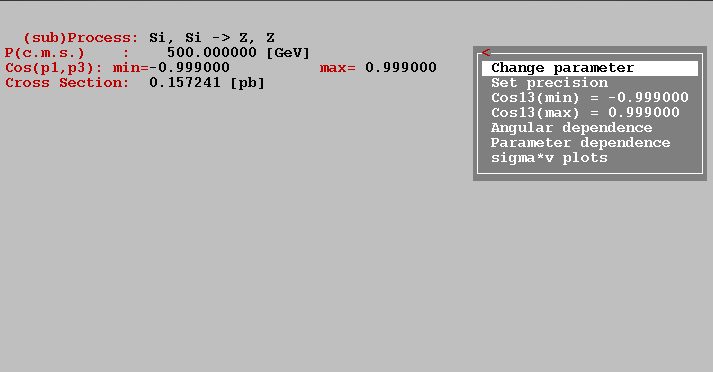
\includegraphics[width=0.5\textwidth]{Sebastian_fig02.png}
	\caption{CalcHEP Calculos.}
	\label{fig:fig01}
\end{figure}

\section{Copyright}

\includegraphics[scale=0.5]{cc} Creative Commons Attribution-Share Alike 3.0 United States License.


%REFERENCIAS ================================================================================

\begin{thebibliography}{}
\bibitem[1]{Goud} Goudelis A., Mambrini Y., Yaguna C., \textit{Antimatter signals of singlet scalar dark matter}. 2009. ArXiv:0909.2799v2 [hep-ph]
\bibitem[2]{profe} Restrepo D., \textit{Notas del curso de mecánica cuántica relativista}. 2011.
\bibitem[3]{lah} Lahiri A., Palash B. P. \textit{A first book of Quantum Field Theory 2ed}. 2005. Alpha Science International Ltd.
\end{thebibliography}


%%% Local Variables: 
%%% mode: latex
%%% TeX-master: "qft_samples"
%%% End: 
